\documentclass[12pt,letterpaper]{article}
\usepackage{geometry} % see geometry.pdf on how to lay out the page. There's lots.
%\geometry{a4paper} % or letter or a5paper or ... etc
% \geometry{landscape} % rotated page geometry

%% LaTeX - Article customise

%%% PACKAGES
\usepackage{booktabs} % for much better looking tables
\usepackage{array} % for better arrays (eg matrices) in maths
\usepackage{paralist} % very flexible & customisable lists (eg. enumerate/itemize, etc.)
\usepackage{verbatim} % adds environment for commenting out blocks of text & for better verbatim
\usepackage{subfigure} % make it possible to include more than one captioned figure/table in a single float
% These packages are all incorporated in the memoir class to one degree or another...

%%% PAGE DIMENSIONS
\usepackage{geometry} % to change the page dimensions
%\geometry{margins=2cm} % for example, change the margins to 2 inches all round
%\geometry{landscape} % set up the page for landscape
% read geometry.pdf for detailed page layout information

%%% HEADERS & FOOTERS
\usepackage{fancyhdr} % This should be set AFTER setting up the page geometry
\pagestyle{fancy} % options: empty , plain , fancy
\renewcommand{\headrulewidth}{0pt} % customise the layout...
\lhead{}\chead{}\rhead{}
\lfoot{}\cfoot{\thepage}\rfoot{}

%%%% SECTION TITLE APPEARANCE
%\usepackage{sectsty}
%\allsectionsfont{\sffamily\mdseries\upshape} % (See the fntguide.pdf for font help)
%% (This matches ConTeXt defaults)

%% LaTeX Preamble - Common packages

\usepackage[utf8]{inputenc} % Any characters can be typed directly from the keyboard, eg éçñ
\usepackage{textcomp} % provide lots of new symbols
\usepackage{graphicx}  % Add graphics capabilities
%\usepackage{epstopdf} % to include .eps graphics files with pdfLaTeX
\usepackage{flafter}  % Don't place floats before their definition
%\usepackage{topcapt}   % Define \topcation for placing captions above tables (not in gwTeX)
\usepackage{natbib} % use author/date bibliographic citations

\usepackage{amsmath,amssymb}  % Better maths support & more symbols
\usepackage{bm}  % Define \bm{} to use bold math fonts

\usepackage[pdftex,bookmarks,colorlinks,breaklinks]{hyperref}  % PDF hyperlinks, with coloured links
%\definecolor{dullmagenta}{rgb}{0.4,0,0.4}   % #660066
%\definecolor{darkblue}{rgb}{0,0,0.4}
%\hypersetup{linkcolor=red,citecolor=blue,filecolor=dullmagenta,urlcolor=darkblue} % coloured links
%%\hypersetup{linkcolor=black,citecolor=black,filecolor=black,urlcolor=black} % black links, for printed output

\usepackage{memhfixc}  % remove conflict between the memoir class & hyperref
% \usepackage[activate]{pdfcprot}  % Turn on margin kerning (not in gwTeX)
\usepackage{pdfsync}  % enable tex source and pdf output syncronicity

% Defining Itemized List Levels
\renewcommand{\labelitemi}{$-$}
%\renewcommand{\labelitemii}{$\cdot$}
%\renewcommand{\labelitemiii}{$\diamond$}
%\renewcommand{\labelitemiv}{$\ast$}

% Better margins
\usepackage{fullpage}

% Matlab code includer
% load package with ``framed'' and ``numbered'' option.
\usepackage[framed,numbered,autolinebreaks,useliterate]{mcode}

%%% BEGIN DOCUMENT
\begin{document}

% Maybe \noindent

\begin{center}
\huge
NTRT Scaling Analysis work\\
\normalsize
\vspace{0.1in}
Andrew P. (Drew) Sabelhaus\\
apsabelhaus@berkeley.edu \\
14 July 2014
\end{center}

%\vspace{-1em}

This short white paper illustrates the scaling analysis that needs to be done on an NTRT-like system.
This work is designed to convince NTRT/Bullet users that current scaling techniques work in some circumstances, but may have to be modified elsewhere (see: scaling of forces, scaling of angular vs. longitudinal spring constants.)
First, we introduce a simple example system for analysis, then do the nondimensionalization of parameters, and evaluate which scalings need to occur.
Then, simulations of the example system are shown under these scaling conditions.
Once this has been established, the anaysis is put in the context of NTRT simulations, and we show why current simulations have (luckily) worked.
Finally, suggestions are made for generalizing these concepts to new parameters in the simulator.

\section{Example system, angular spring/damper}

In this example system, there is a rod on a hinge (hinge at (x,y) = (0,0) ) with length $l$.
There is an angular (rotational) spring, and an angular damper, acting at the origin also.
Gravity is present, and we assume it acts fully at the center of mass for the rod.

NOTE that this is NOT the same as the longitudinal/linear spring models that are used in NTRT.
This specific system model is analysed first to emphasize that current assumptions don't work.
See later sections for applications to our specific model, once you've convinced yourself that this dimensionless term analysis is necessary.

With the state variables for this system as the angle between the rod and the horizontal, and its derivative,

\[
x = [\theta, \dot \theta]^\top
\]

We can derive the following system dynamics. 
(Note, these are NOT needed for scaling analysis, but are just provided for reference in case you'd like to simulate this yourself to check this math. I did!)

\[
\sum T = I \ddot \theta, \quad \sum T = T_s - T_d + T_g
\]

...where these torques are for the angular spring and damper, and the gravitational force. Their magnitudes are

\[
T_s = k_{\theta}(\theta - \theta_r), \quad T_d = c_{\theta} \dot \theta, \quad T_g = (mg)(r) = \frac{mgl}{2} cos \theta
\]

Here, $\theta_r$ is the rest angle of the spring. So, then, our rigid body dynamics are

\[
\ddot \theta = \frac{1}{I} (\frac{mgl}{2} cos \theta + k_{\theta} \theta - k_{\theta} \theta_r - c_{\theta} \dot \theta )
\]

For a solid rod,
\[
I = \frac{m l^3}{3}
\]

And the full dynamics equation is
\[
\ddot \theta = \frac{3}{m l^3} (\frac{mgl}{2} cos \theta + k_{\theta} \theta - k_{\theta} \theta_r - c_{\theta} \dot \theta )
\]

We will not return to this for the rest of the analysis, but it's useful for reference.

\section{$\Pi$ Terms and Nondimensional Numbers}

I won't include a discussion/justification of NDMs here, see other work for that discussion - e.g. the undergrad fluids textbook by Munsen.
It's sufficient to recount the following theorem, the Buckingham Pi Theorem, which states, loosely: \\


Given a system with $n$ variables and parameters, of which there are $k$ underlying basic units (phenomena), construct exactly $n-k$ nondimensional numbers.
Then, if the magnitudes of each of these dimensionless numbers is kept the same under scaling of some of the parameters, via scaling other parameters equivalently, then the kinematic and dynamic responses of the original system and the scaled system will be $similar$ (e.g. equal.) \\


Usually, $n$ includes both constants in the system as well as anything else that one might care about, such as initial conditions or output results (forces, trajectories.)
Also, for physical rigid body dynamics, $k$ is almost always the set of $\{Mass, Length, Time\}$ or $M, L, T$, so $k=3$ moving forward.

\subsection{System variables and units}

The above example system has the following parameters and variables (both implicit and explicit) and the following units:

\[
\text{mass:} \quad m \sim M^1
\]
\[
\text{spring rest angle:} \quad \theta_r \sim 0 \text{, because radians!}
\]
\[
\text{length of rod:} \quad l \sim L^1
\]
\[
\text{gravitational acceleration:} \quad g \sim L^1 T^{-2}
\]
\[
\text{angular spring constant:} \quad k_{\theta} \sim M^1 T^{-2} L^1 
\]
\[
\text{angular damping coefficient:} \quad c_{\theta} \sim M^1 T^{-1} L^1
\]
\[
\text{force:} \quad  F \sim M^1 L^1 T^{-2}
\]
\[
\text{time:} \quad t \sim T^1
\]

These were derived with force in Newtons, $kg*m/s^2$.

Note that, unlike with longitudinal springs and dampers, their angular counterparts DO have a length dependence! This becomes important in a minute...

\subsection{Generation of $\Pi$-Terms}

In order to make use of Buckingham's Pi Theorem to scale our system correctly, we need to make $n-k = 8-3 = 5$ pi terms. I won't do that many until needed for illustrating a concept - I'll show the errors this generates as they occur.

The first step in this procedure is to select $k=3$ ``repeating variables,'' which will make up our pi terms. Any subset of 3 is fine here, under the following conditions:

1. The set of repeating variables must not be able to make a nondimensional set by themselves (i.e. they must be an independent basis)

2. Avoid selecting difficult-to-scale variables as repeaters (e.g. don't choose time here because that's hard)


Let's choose, in this example, our repeaters as $m, l, c$. See the Munsen textbook (or other resources) to see how to procedurally derive all the pi terms. 
Skipping ahead, here are the ones I derived.
You can check the units in all of these: they divide out evenly.

\[
\Pi_1 = \Pi_{\theta_r} = 0
\]
\[
\Pi_2 = \Pi_{g} = \frac{gm^2l}{c_{\theta}^2}
\]
\[
\Pi_3 = \Pi_{k_{\theta}} = \frac{m l k_{\theta}}{c_{\theta}^2}
\]

\subsection{$\Pi$-Term Analysis for Scaling}

So, if for this system, we want to scale gravitional acceleration by a factor $s$, such that

\[
g_2 = (s) (g_1)
\]

We would also need to scale length of rod (because of $\Pi_2$) and angular spring constant (because of $\Pi_3$) by the following:

\[
k_{\theta_2} = (s) k_{\theta_1}, \quad \quad l_2 = \frac{1}{s} l_1
\]

However, there are other combinations we could choose! Pi term scalings are not unique. Here is another set of scaling factors we could choose, again assuming we want to scale gravity by $s$.

\[
%m_{2} = \frac{1}{\sqrt{s}} m_{1}, \quad \quad l_2 = (\sqrt{s}) l_1
k_{\theta_2} = (s) k_{\theta_1}, \quad \quad c_{\theta_2} = (\sqrt{s}) c_{\theta_1}
\]

...and we could come up with others involving the damping term, or involving all of them, if we wanted to. By the theorem, these scalings should all give us the same result.

\section{Simulation of scaled systems}

Figures \ref{fig:original_angular} and \ref{fig:grav_only_angular} shows simulations of the original system, under parameters defined in the accompanying MATLAB file, as well as one with only gravity scaled by a constant (which is expected to yield a quantitatiely different result.)
Here, the scaling factor was $s=2$.
Figure \ref{fig:l_g_angular} shows a simulation with length scaled with gravity, as per the naive assumption suggested by Bullet developers.
This one is done with proportional scaling: gravity multiplied by $s$, length multiplied by $s$.
However, to head off complaints, I've also included a plot where length is multiplied by $1/s$ in figure \ref{fig:l_g_inverse_angular}.
Both can be seen as incorrect scalings.

Figures \ref{fig:k_l_g_angular} and \ref{fig:m_l_g_angular} show two simulations of ``properly scaled'' systems under the two different parameter transformations listed above.
In order to see differences in the following plots, pay attention to the magnitude of the first peak, as well as the settling time.

\begin{figure}[ht]
  \centering
  \includegraphics[width=.48\linewidth]{img/original_angular.eps}
  \caption{Original system, no scaling. }
  \label{fig:original_angular}
\end{figure}

\begin{figure}[ht]
  \centering
  \includegraphics[width=.48\linewidth]{img/grav_only_angular.eps}
  \caption{System with gravity scaled by 2. }
  \label{fig:grav_only_angular}
\end{figure}

\begin{figure}[ht]
  \centering
  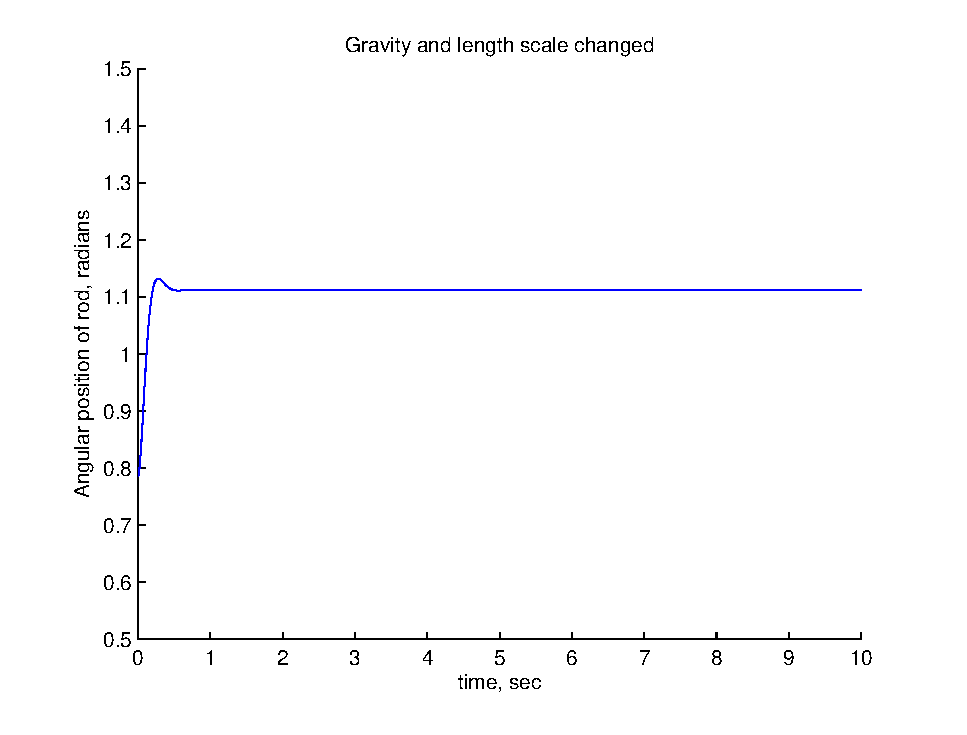
\includegraphics[width=.48\linewidth]{img/l_g_angular.eps}
  \caption{System with length scaled as well as gravity, both proportional with $s$. }
  \label{fig:l_g_angular}
\end{figure}

\begin{figure}[ht]
  \centering
  \includegraphics[width=.48\linewidth]{img/l_g_inverse_angular.eps}
  \caption{System with length scaled as well as gravity, inversely: gravity with $s$, length with $1/s$. }
  \label{fig:l_g_inverse_angular}
\end{figure}

\begin{figure}[ht]
  \centering
  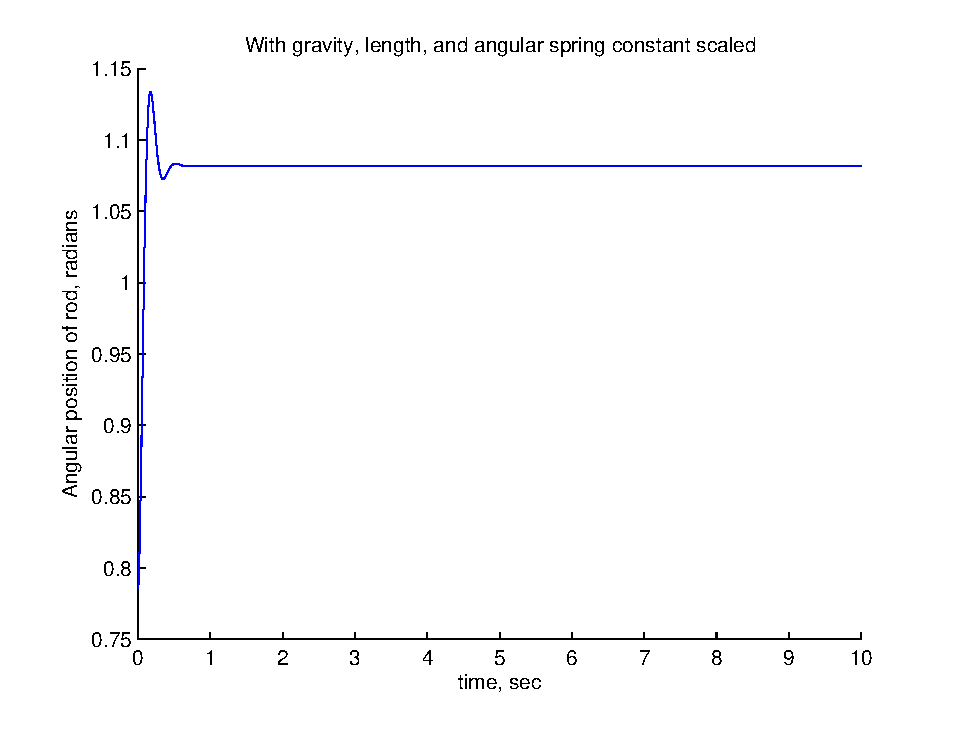
\includegraphics[width=.48\linewidth]{img/k_l_g_angular.eps}
  \caption{System with gravity, angular spring constant, and length scaled. }
  \label{fig:k_l_g_angular}
\end{figure}

\begin{figure}[ht]
  \centering
  \includegraphics[width=.48\linewidth]{img/k_c_g_angular.eps}
  \caption{System with gravity and angular spring/damping constants scaled. }
  \label{fig:k_c_g_angular}
\end{figure}


What happened? Plots \ref{fig:k_l_g_angular} and \ref{fig:k_c_g_angular} are NOT equivalent to the orignal in figure \ref{fig:original_angular}! 
For plot \ref{fig:k_l_g_angular} there is likely something that I'm doing wrong with my simulation - I can't quite figure out why it's coming out like this.
It's included for reference for someone else to figure out later if so desired.


But, plot \ref{fig:k_c_g_angular} is expected, as per the analysis below.
We messed up - we're not following the theorem exactly! 
We conveniently left out the two remaining Pi terms of force and time. 
Let's see if including these compels us to change our scalings.
After some algebra, these two Pi terms are

\[
\Pi_4 = \Pi_{F} = \frac{fill in later}{fill in later}
\]
\[
\Pi_5 = \Pi_{t} = \frac{tc_{\theta}}{ml}
\]

Ack! The time scaling! 
This gets complicated now: let's find a scaling that keeps time consistent also.
Remember that time gets difficult for us to scale: we could do it post-hoc after the simulation, but that's a pain, so let's see if we can just change the constants.

...

...and it looks like this system of equations is unsolvable unless we scale time too. Darn. 
Here's a scaling with time, based on the original scaling:

\[
k_{\theta_2} = (s) k_{\theta_1}, \quad \quad c_{\theta_2} = (\sqrt{s}) c_{\theta_1}, \quad \quad t_2 = \frac{1}{\sqrt{s}} t_1
\]

This system is simulated in figure \ref{fig:k_c_t_g_angular}. See how this is the same result as figure \ref{fig:original_angular}, finally!

\begin{figure}[ht]
  \centering
  \includegraphics[width=.48\linewidth]{img/k_c_t_g_angular.eps}
  \caption{System with gravity, angular spring and damping constants, and time scaled. }
  \label{fig:k_c_t_g_angular}
\end{figure}

In conclusion, this section should show by contradiction that the following two statements are untrue: \\

1. Commutativity of multiplication implies that we only need to scale length when scaling gravity: 
$n * (length / time^2) == (n * length) / time^2.$

If this were true, not only would figures \ref{fig:original_angular} and \ref{fig:l_g_angular} be identical, but there wouldn't be a need for dimensional analysis in the first place.
The fact that the Buckingham Pi theorem exists in the first place really disproves this idea intuitively. \\

2. Instead of simulating a robot of characteristic size l, mass m in and gravity g, we simulate a robot of size 10*l, mass m and gravity 10*g.
The resulting large robot has identical behavior to the original small robot, except for a multiplicative factor 10 for units which depend linearly on length, 100 for units which depend quadratically on length and so on.

This is not true, since we may need to pay attention to ALL variables at play. Some (seemingly unrelated) ones may cause significant changes in the reqiured dimensionless terms, as explained in the next section on why our simulations currently ''work''. 

\section{Analysis of related longitudinal spring/damper systems, for NTRT use}

The above analysis is based on a system where parameters are angular.
However, our simulated systems use longitudinal/linear dampers and springs, and the analysis changes quite a bit.
This is somewhat unexpected at first - why would the units of these extra parameters influence the required scaling for unrelated terms? - but by the Pi theorem, it must work this way. \\

Ignoring a full dynamics derivation (no more simulations for me!), let's take the following constitutive equations for longitudinal springs and dampers:

\[
F_s = k(x - x_r), \quad F_d = c \dot x
\]

So, here is how the units and Pi terms would change for a longitudinal spring/damper system:

\[
\text{spring rest length:} \quad x_r \sim L^1
\]
\[
\text{spring constant:} \quad k \sim M^1 T^{-2}
\]
\[
\text{damping coefficient:} \quad c \sim M^1 T^{-1}
\]

Note the missing length scale in $k$ and $c$. 
This is because, for example, $k$ needs to be units of $N/m$ instead of $N/rad$, and the extra length term cancels out.
The new Pi terms, using the same set of $\{m,l,c\}$ are:

\[
\Pi_1 = \Pi_{x_r} = \frac{x_r}{l}
\]
\[
\Pi_2 = \Pi_{g} = \frac{gm^2}{c^2l}
\]
\[
\Pi_3 = \Pi_{k} = \frac{km}{c^2}
\]
\[
\Pi_4 = \Pi_{F} = \frac{Fm}{c^2l}
\]
\[
\Pi_5 = \Pi_{t} = \frac{tc}{m}
\]

Note that here, the scaling of gravity with length DOES actually work!
When $g$ is multiplied by $s$, we can do the same to $l$, then to $x_r$ by $\Pi_1$ and to $F$ by $\Pi_4$.
The takeaway here is that without extra Pi terms for more parameters like $k_{\theta}$, we can get away with this simple scaling, BUT we need to be careful and re-evaluate our Pi terms each time a new unit parameter is introduced.

\section{Scaling Analysis for General Linear Systems}

Finally, I'll finish with an argument as to why a truly linear system would not need any of this scaling analysis.
I originally tried these simulations using a simple spring-mass-damper vertically oriented under gravity, e.g.

\[
m \ddot x + c \dot x + k x = mg
\]

With this system, the ''gravity proportional to length'' scaling also works, but for an entirely different reason.
What's actually going on in this case is a change in the magnitude of the input-output transfer function, and so the scaling ITSELF is non-dimensional!
One way to see this is to notice that the gravitational force is time-invariant, and could thus be replaced by a step input:

\[
m \ddot x + c \dot x + k x = u(t)
\]

By superposition of linear systems, the magnitude of the output of the system of

\[
m \ddot x + c \dot x + k x = (n) u(t)
\]

...will be exactly $n$ times larger. Thus, dividing the output by $n$ re-scales to the proper dimensions.
I'm lazy and don't feel like looking up the theorems here, but it should be easy to justify if so desired.

\section{Moving Forward}

So, after all this work, where do we stand? 

First, we need to check NTRT and Bullet for other parameters with other units, create Pi terms for them, and check to be absolutely sure we have the required number of dimensionless numbers.
Coefficients that are dimensionless can be left out, so I'm not aware of other constants that would need to be scaled, but it's worth a hard look nonetheless.
We should list all these, their corresponding Pi terms, and post the analysis somewhere so we can justify we're scaled correctly.

Second, we should look through old results and make sure we scaled (for example) output forces after the simulation.
This would be relevant for the IPPW paper and Atil's learning results with the original SUPERball model.

Third, we should alert users to situations where their scaling might get crazy messy, and things to watch out for.
Two situations come to mind.
As one example, developing a model-based controller with parameters calculated analytically would have to be scaled. A controller using nonlinear damping techniques would require a complete re-derivation of these Pi terms and scaling.
Another situation would be the creation of a new NTRT object, like a new model, which has constitutive equations that use new constants and terms.
One example here would be the new string model that Brian Tietz Mirletz is working on.

Finally, all of this should be formalized and integrated into Bullet and/or NTRT in as scalable a way as possible.
I'm not sure if there are automated techniques to developing Pi terms and scaling (?), but if those exist, it would be great to explore them.
Nonetheless we need to write good code to perform these scalings behind-the-scene.

If anyone would like to run my MATLAB code (attached in this directory), it should be straightforward, but email me if you find issues.

\end{document}
